\documentclass[a4paper,12pt]{article} % тип документа

% Поля страниц
\usepackage[left=2.5cm,right=2.5cm, top=2cm,bottom=2cm,bindingoffset=0cm]{geometry}
    
%Пакет дял таблиц   
\usepackage{multirow} 
    
%Отступ после заголовка    
\usepackage{indentfirst}


% Рисунки
\usepackage{subcaption,floatrow,graphicx,calc}
\usepackage{wrapfig}

% Создаёем новый разделитель
\DeclareFloatSeparators{mysep}{\hspace{1cm}}

% Ссылки?
\usepackage{hyperref}
\usepackage[rgb]{xcolor}
\hypersetup{				% Гиперссылки
    colorlinks=true,       	% false: ссылки в рамках
	urlcolor=blue          % на URL
}


%  Русский язык
\usepackage[T2A]{fontenc}			% кодировка
\usepackage[utf8]{inputenc}			% кодировка исходного текста
\usepackage[english,russian]{babel}	% локализация и переносы


% Математика
\usepackage{amsmath,amsfonts,amssymb,amsthm,mathtools, mathrsfs, wasysym}


\begin{document}
\begin{center}
	\footnotesize{ФЕДЕРАЛЬНОЕ ГОСУДАРСТВЕННОЕ АВТОНОМНОЕ ОБРАЗОВАТЕЛЬНОЕ 			УЧРЕЖДЕНИЕ ВЫСШЕГО ОБРАЗОВАНИЯ}\\
	\footnotesize{МОСКОВСКИЙ ФИЗИКО-ТЕХНИЧЕСКИЙ ИНСТИТУТ\\(НАЦИОНАЛЬНЫЙ 			ИССЛЕДОВАТЕЛЬСКИЙ УНИВЕРСИТЕТ)}\\
	\footnotesize{ФАКУЛЬТЕТ ОБЩЕЙ И ПРИКЛАДНОЙ ФИЗИКИ\\}
	\hfill \break
	\hfill\break
	\hfill\break
	\hfill \break
	\hfill \break
	\hfill \break
	\hfill \break
	\hfill \break
	\hfill \break
	\hfill \break
	\hfill \break
	\hfill \break
	\hfill \break
	\hfill \break
	\large{Лабораторная работа № 5.5.1 \\\textbf{Измерение коэффициента ослабления потока $\gamma$-лучей в веществе и опредление их энерегии.}}\\
	\hfill \break
	\hfill \break
	\hfill \break
	\begin{flushright}
		Серебренников Даниил\\
		Группа Б02-826м
	\end{flushright}
	\hfill \break
	\hfill \break
	\hfill \break
	\hfill \break
	\hfill \break
	\hfill \break
	\hfill \break
	\hfill \break
	\hfill \break
	\hfill \break
	\hfill \break
\end{center}
\begin{center}
	Долгопрудный, 2020 г.
\end{center}
\thispagestyle{empty}
\newpage
	\textbf{Цель работы:} c помощью сцинтилляционного счетки измерить линейные коэффициенты ослабления потока $\gamma$-лучей в свинце, железе и алюминии; по их велечине определить энергию $\gamma$-квантов.

\section{Теоретическая часть}
	Гамма-лучи возникают при переходе возбужденных ядер из одного энергетического состояния в другое, более низкое. Энергия $\gamma$-квантов обычно заключена между несколькими десятками килоэлектронвольт и несколькими миллионами электрон-вольт. Гамма-кванты не несут электрического заряда, их масса равна нулю. Проходя, через вещество, пучок $\gamma$-квантов постепенно ослабляется. Ослабление просходит по експоненциальному закону, который может быть записан в следующей форме:
	\begin{equation}
		\label{eq1}
		I = I_0 e^{-\mu l},
	\end{equation}
	где $I$, $I_0$ -- интенсивности прошедшего и падающего излучений; $l$ -- длина пути, пройденного пучком $\gamma$-лучей; $\mu$ -- коэффициент ослабления потока в веществе.
	
	Ослабление потока $\gamma$-лучей, происходящее при прохождении среды, связано с тремя эффектами: фотоэлектрическим поглощением, комптоновским рассеянием и с генерацией электрон-позитронных пар.
	
	В случае опытов, поставленных в хорошей геометрии, при прохождении $\gamma$-лучей через вещество меняет только количество, но не энергия $\gamma$-квантов в пучке, так что коэффициент $\mu$, характеризующий поглощение $\gamma$-квантов в веществе, не зависит от длины пути. Обозначим через $-dN$ число $\gamma$-квантов, выбывших их пучка на пути $dl$. Это число пропорционально имеющемуся их числу $N$ и пройденному пути $dl$. Cледовательно,
	\begin{equation}
		\label{eq2}
		-dN = \mu N \, dl.
	\end{equation} 
	Интегрируя уравнение~(\ref{eq2}) от нулевой толщины до заданной, получим
	\begin{equation}
		\label{eq3}
		N = N_0 e^{-\mu l}.
	\end{equation}

	Вообще говоря, в плохой геометрии, когда рассеянные под небольшими углами $\gamma$-кванты остаются в пучке, их спектр с прохождением вещества меняется, поэтому формула~(\ref{eq1}) непреминима. Однако в этом случае она работает лучше, чем можно было ожидать.
	
	В данной работе коэффициент ослабления $\mu$ измеряется в хорошей геометрии. Из формулы~(\ref{eq3}) имеем:
	\begin{equation}
		\tag{$\star$}
		\label{formula}
		\mu = \frac{1}{l} \ln \frac{N_0}{N}.
	\end{equation}

	Для определения коэффициента ослабления нужно, таким образом, измерить толщтну образца $l$, число падающих частиц $N_0$ и число частиц $N$, прошедших через образец.
	
\newpage
\section{Экспериментальная установка}
	Схема установки, исползуемой в работе, показана на рис.~\ref{fig:ustanovka1}. Свинцовый коллиматор выделяет узкий почти параллельный пучок $\gamma$-квантов, проходящий через набор поглотителей П и регистрируемый сцинтиляцонным счетчиком. Сигналы от счетчика усиливаются и регистрируются пересчетным прибором ПП. Высоковольтный выпрямитель ВВ обеспечивает питание сцинтилляционного счетчика.
	
	\begin{figure}[h!]
		\begin{floatrow}
			\ffigbox[\FBwidth]{\caption{Блок-схема установки, используемой для измерения коэффициентов ослабления потока $\gamma$-лучей.}\label{fig:ustanovka1}}%
			{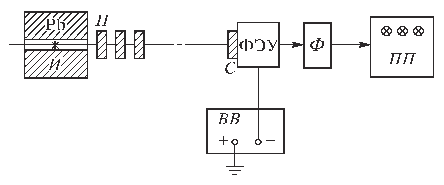
\includegraphics[scale=1.5]{ustanovka1.pdf}}    
		\end{floatrow}
	\end{figure}

	При недостаточно хорошей геометрии в результаты опытов могут вкрасться существенные погрешности. В реальных установках всегда имеется конечная вероятность того, что $\gamma$-квант провзаимодействует в поглотителе несколько раз до того, как попадет в детектор (пути таких квантов показаны на рис.~\ref{fig:ustanovka2}). Чтобы уменьшить число таких случаев, в данной работе сцинтилляционный счетчик расположен на большом расстоянии от источиника $\gamma$-квантов, а поглотители имеют небольшие размеры. Их следует устанавливать за коллиматорной щелью на некотором расстоянии друг от друга, чтобы испытавшие комптоновское рассеяние и выбывшие из прямого потока кванты с меньшей вероятностью могли в него вернуться.

	\begin{figure}[h!]
		\begin{floatrow}
			\ffigbox[\FBwidth]{\caption{Схема рассеяния $\gamma$-квантов в поглотителе.}\label{fig:ustanovka2}}%
			{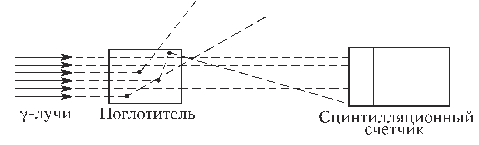
\includegraphics[scale=1.5]{ustanovka2.pdf}}    
		\end{floatrow}
	\end{figure}
	
	
	
	\newpage
	\section{Экспериментальные данные}
		В условиях нашего эксперимента необходимо учитывать фон, поэтому
		\begin{equation*}
			N_0 = n_0 - n_\text{фон}, \ N = n - n_\text{фон}.
		\end{equation*}
		
		
		\floatsetup[table]{capposition=top}	
		\begin{table}[H]
			\caption{Измерение фона и потока $\gamma$-излучения в воздухе.}
			\label{table:exp1}
			\begin{tabular}{|c|c|c|}
				\hline
				& $t$, с & $n$    \\ \hline
				$n_{\text{фон}}$ & 100    & 1708   \\ \hline
				$n_0$            & 60     & 814085 \\ \hline
			\end{tabular}
		\end{table}
		
		
	
		\floatsetup[table]{capposition=top}	
		\begin{table}[H]
			\caption{Результаты измерений.}
			\label{table:exp2}
			\begin{tabular}{|c|c|c|c|c|c|c|c|c|c|c|c|}
				\hline
				\multicolumn{3}{|c|}{Алюминий} & \multicolumn{3}{c|}{Железо} & \multicolumn{3}{c|}{Свинец} & \multicolumn{3}{c|}{Вещество <<X>>} \\ \hline
				$l$, см   & $t$, с   & $n$     & $l$, см  & $t$, с  & $n$    & $l$, см  & $t$, с  & $n$    & $l$, см     & $t$, с    & $n$       \\ \hline
				2,00      & 100      & 869822  & 1,02     & 100     & 750826 & 0,52     & 100     & 755789 & 1,97        & 60        & 803585    \\ \hline
				4,01      & 100      & 582734  & 2,03     & 100     & 424457 & 0,96     & 100     & 455240 & 3,92        & 60        & 786234    \\ \hline
				6,02      & 100      & 385059  & 3,04     & 100     & 240069 & 1,45     & 100     & 256403 & 5,91        & 60        & 768022    \\ \hline
				8,06      & 100      & 257977  & 4,04     & 100     & 136849 & 1,95     & 100     & 148530 & 7,92        & 60        & 749618    \\ \hline
				10,06     & 100      & 172747  & 5,05     & 100     & 80397  & 2,47     & 100     & 84818  & 9,78        & 60        & 729570    \\ \hline
			\end{tabular}
		\end{table}
	
		 Отметим, что при повторном проведении опытов результаты измерений количества частиц $n$ отличались в среднем на 5\% от значений в табл.~\ref{table:exp2}. Поэтому относительная погрешность $n$ будет порядка 5\%. Длина $l$ была измерена достаточно точно штангенциркулем и $\sigma_l / l < 1\%$, где $\sigma_l = 0,01$ см.
		 
		 
	\newpage
	\section{Обработка результатов}
		Для определения коэффициента ослабления $\mu$ в различных веществах небходимо построить графики  зависимостей $\ln N_0/N$ от $l$. Погрешность вычисления натурального логарифма можно оценить следующим образом:
		\begin{equation*}
			\sigma_{\ln} = \frac{1}{N_0/N} \sigma_{N_0/N} = \sqrt{\left(\frac{\sigma_{N_0}}{N_0}\right)^2+\left(\frac{\sigma_{N}}{N}\right)^2} \approx \sqrt{\left(\frac{\sigma_{n_0}}{n_0}\right)^2+\left(\frac{\sigma_{n}}{n}\right)^2} = 0,05\sqrt{2} \approx 0,07.
		\end{equation*}
		
		\floatsetup[table]{capposition=top}	
		\begin{table}[H]
			\caption{Результаты вычислений.}
			\label{table:exp3}
			\begin{tabular}{|c|c|c|c|c|c|c|c|}
				\hline
				\multicolumn{2}{|c|}{Алюминий} & \multicolumn{2}{c|}{Железо} & \multicolumn{2}{c|}{Свинец} & \multicolumn{2}{c|}{Вещество <<X>>} \\ \hline
				$l$, см    & $\ln N_0/N$, с    & $l$, см   & $\ln N_0/N$, с  & $l$, см   & $\ln N_0/N$, с  & $l$, см       & $\ln N_0/N$, с      \\ \hline
				2,00       & 0,45              & 1,02      & 0,59            & 0,52      & 0,59            & 1,97          & 0,01                \\ \hline
				4,01       & 0,85              & 2,03      & 1,16            & 0,96      & 1,09            & 3,92          & 0,03                \\ \hline
				6,02       & 1,26              & 3,04      & 1,74            & 1,45      & 1,67            & 5,91          & 0,06                \\ \hline
				8,06       & 1,67              & 4,04      & 2,31            & 1,95      & 2,22            & 7,92          & 0,08                \\ \hline
				10,06      & 2,07              & 5,05      & 2,85            & 2,47      & 2,79            & 9,78          & 0,11                \\ \hline
			\end{tabular}
		\end{table} 
	
		По данным таблицы~\ref{table:exp3} были построены прямые (рис. \ref{fig:graph}), наклоны которых согласно формуле~(\ref{formula}) есть линейные коэффициенты ослабления $\mu$ потока $\gamma$-излучения в веществе.
	
		\begin{figure}[h!]
			\begin{floatrow}
				\ffigbox[\FBwidth]{\caption{Графики зависимостей $\ln N_0/N$ от $l$ для различных материалов.}\label{fig:graph}}%
				{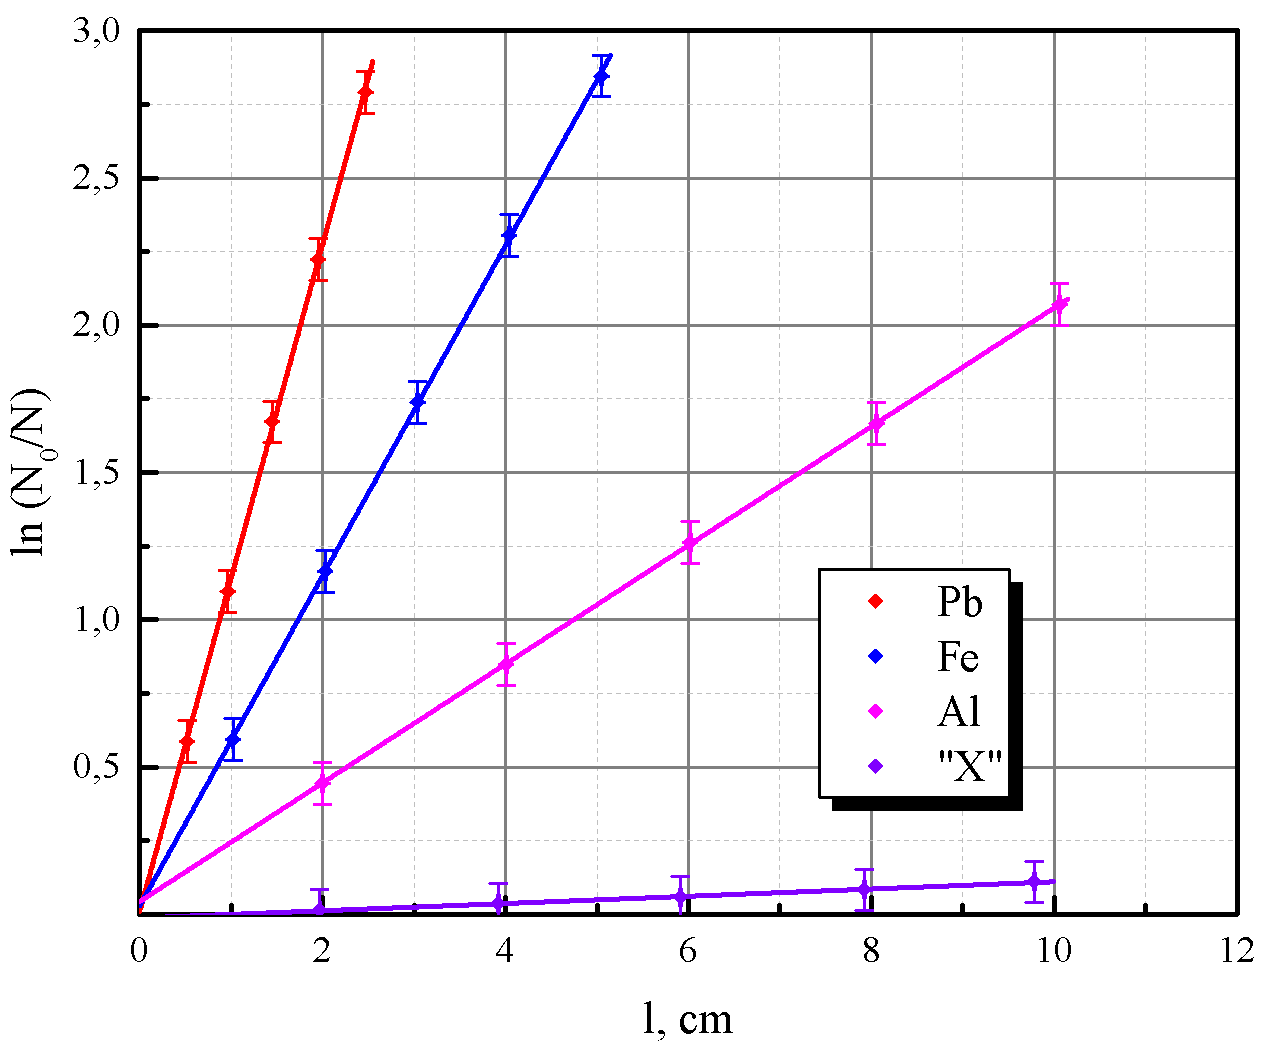
\includegraphics[scale=0.5]{graph1.pdf}}     
			\end{floatrow}
		\end{figure}
		
		Имеем:
		\floatsetup[table]{capposition=top}	
		\begin{table}[H]
			\caption{Наклоны прямых.}
			\label{table:final}
			\begin{tabular}{|c|c|c|c|c|}
				\hline
				& Pb          & Fe         & Al             & X              \\ \hline
				$\mu$, $10^{-3}\cdot \text{см}^{-1}$ & $1132\pm11$ & $561\pm 4$ & $201,7\pm 0,7$ & $12,3 \pm 0,4$ \\ \hline
			\end{tabular}
		\end{table}
	
\newpage
\section{Обсуждение результатов и выводы}
	В настоящей лабораторной работе с помощью сцинтилляционного счетчика были измерены (табл.~\ref{table:final}) линейные коэффициенты ослабления $\mu$ потока $\gamma$-лучей в свинце, железе, алюминии и в некотором веществе <<X>>, которое внешне напоминало дсп. Среднюю энергию излучения, испускаемого источником, можно определить по следующей справочной таблице, приведенной в приложении лабораторного практикума по общей физике <<Квантовая физика>>:
	\floatsetup[table]{capposition=top}	
	\begin{table}[H]
		\caption{Коэффициенты поглощения $\gamma$-лучей в различных веществах (в~см$^{-1}$).}
		\label{table:spravocka}
		\begin{tabular}{|c|c|c|c|c|}
			\hline
			$E_\gamma$, МэВ & Pb    & Fe    & Al    & <<X>> \\ \hline
			0,6             & 1,349 & 0,605 & 0,210 & -     \\ \hline
			0,8             & 0,982 & 0,526 & 0,184 & -     \\ \hline
		\end{tabular}
	\end{table}

	Видно, что полученные нами значения коэффициента ослабления потока $\mu$ для каждого вещества лежат в диапазоне энергий от 0,6 МэВ до 0,8 МэВ, поэтому средняя энергия излучения есть $E_\gamma = 0,7$ МэВ.
	
	Заметим, что наклоны прямых на рис.~\ref{fig:graph} по мере роста заряда ядра увеличиваются. Это связано с природой ослабления $\gamma$-лучей при их прохождении в веществе: фотоэлектрическое поглощение, комптоновское рассеяние, генерация электрон-позитронных пар. Так как $E_\gamma = 0,7 \ \text{МэВ} < 2mc^2$ = 1,02 МэВ, то в нашем случае фотон не может превратиться в электрон-позитронную пару. Комптоновское рассеяние происходит на свободных или слабосвязанных электронах, поэтому, очевидно, сечение не зависит от заряда ядра, откуда $\mu_k \propto Z$. Фотоэффект же в отличии от Комптоновского рассеяния происходит на атоме, и, естественно, что в этом случае сечение уже будет зависеть от заряда ядра. Вообще говоря, строгий квантово-механический рассчет приводит к результату $\sigma_\text{ф} \propto Z^5$. Таким образом, коэффициент ослабления $\gamma$-лучей должен расти при увеличении заряда ядра. 
	

	
\end{document}